\documentclass{acm_proc_article-sp}

\usepackage[utf8]{inputenc}
\usepackage[T1]{fontenc}
\usepackage{float}
\usepackage{todonotes}
\usepackage{xspace}
\usepackage{tikz}
\usepackage{verbatim}

\usetikzlibrary{decorations.pathmorphing}

\newcommand{\td}[1]{%
  \todo[inline]{#1}%
}

\newcommand{\pfs}{Pinguesco\xspace}
\newcommand{\pfsfs}{PinguescoFS\xspace}

\begin{document}

\title{\pfs: A 32-bit File System}

\numberofauthors{1} 

\author{
  \alignauthor
  Diogo Sousa\\
  \affaddr{Faculdade de Ciências e Tecnologia}\\
  \affaddr{Universidade Nova de Lisboa}\\
  \affaddr{Caparica, Portugal}\\
  \email{dm.sousa@fct.unl.pt}
}

\date{\today}

\maketitle

\begin{abstract}
Permanent storage of structured data is on of the most basic abstractions 
expected from a general purpose operating system. 
File system stored on a disk solve this requirement. 
This paper discusses the design, implementation and
evaluation of \pfs\footnote{Latin for \emph{fat}.}, a simple 32-bit 
file system build on top of \emph{FUSE}.
\end{abstract}

% A category with the (minimum) three required fields
% http://www.acm.org/about/class/ccs98-html
\category{D.4.3}{File Systems Management}{}

\keywords{file system, file allocation table, indirect block, fuse}

\section{Introduction}
This paper presents \pfs, a 32-bit disk file system. This file system
was implemented in \emph{C} with \emph{FUSE}, thus running in \emph{userland}.
The file system partially implements the \emph{POSIX standard}.

\pfsfs support every common operation except permission 
handling, file timestamps and soft- and hard-links, and the data
is permanently stored on a block device.

A file allocation table allows fast block allocation and multiple indirection
blocks are used to support large files. Directories are supported and can
be nested to an arbitrary depth.

\section{Pinguesco File System Design}
The \pfsfs has a simple structure. The \emph{superblock} is the first
block (block 0) and contains a magic number identifying the device
as a \pfs file system, the number of blocks used and the number of inodes.
The superblock also contains a pointer to the first free block.
%% Super Block
%%   position: 0
%%   content:
%%     - magic number         (4 bytes) - 0xbadebabe
%%     - free block list head (4 bytes)
%%     - number of blocks     (4 bytes)
%%     - number of inodes     (4 bytes)

The next $2^{14}=16384$ blocks contain the file allocation table \cite{mos:fs}. 
This table keep a list of free blocks, with the first free block specified
in the superblock. The last free block points to 0. This FAT size
allows the file system to handle $4GB$ of data.
The FAT allows constant time block allocation with no hard drive accesses,
since it is loaded to main memory when the file system is mounted.
%% File Allocation Table
%%   position: 1 .. 16384
%%   content:
%%     - next pointers in the free list

Each file in the file system is represented by an inode. An inode
can represent a directory or a regular file. The inode also keeps
the number of blocks allocated to represent that file, being that
data blocks, indirect blocks or, in case of directories dentry tables 
(explained bellow). If the inode represent a regular file then the number
of bytes the file has is also present in the inode, as well as the pointers
to the indirect blocks. There are three pointers to indirect blocks, with
single indirection, double indirection and triple indirection to allow
for large files. This is done in the same way as the UNIX V7 file system
\cite{mos:fs}.
If the inode represent a directory a pointer to the
first dentry table block is also kept in the inode.
%% Inode structure
%%   position: arbitrary
%%   content:
%%     + type (1 byte)
%%     + dentry block (if the inode is a directory) (4 bytes)
%%     + number of blocks of the file (including inode) (4 bytes)
%%     + size (if the inode is a file) (4 bytes)
%%     + single indirect block (if the inode is a file) (4 bytes)
%%     + double indirect block (if the inode is a file) (4 bytes)
%%     + triple indirect block (if the inode is a file) (4 bytes)

A dentry table represent the content of a directory. This table stores
the filenames and correspondent inode of the directory. Since the number
of files in the directory may be arbitrarily large, at the end of each
dentry table exists a pointer to the next dentry table.
%% Directory entry structure
%%   position: arbitrary
%%   content:
%%     - nul terminated name (64 bytes), inode number (4 bytes) (15 times)
%%     - next pointer (4 bytes)
%%     Note: An unused entry will have a name starting by nul

The indirect blocks are simply a sequence of pointers. The final indirection
level point to the block containing the correspondent data. If this points
to 0 then that block represents a block in which every byte is $0\text{x}00$.
This makes it easy for the expansion of a file with a \verb|truncate| operation.
%% Indirect block structure
%%     - block (4 bytes) (256 times)

The first directory inode is always in the block $16385$, the first block
after the file allocation table.
%% Root inode
%%   position: 16385

Figure \ref{fig:pfsstructex} exemplifies a \pfs File System with a file
called ``foo'' containing the line ``Hello World''.

\begin{figure}[H]
  \begin{center}
    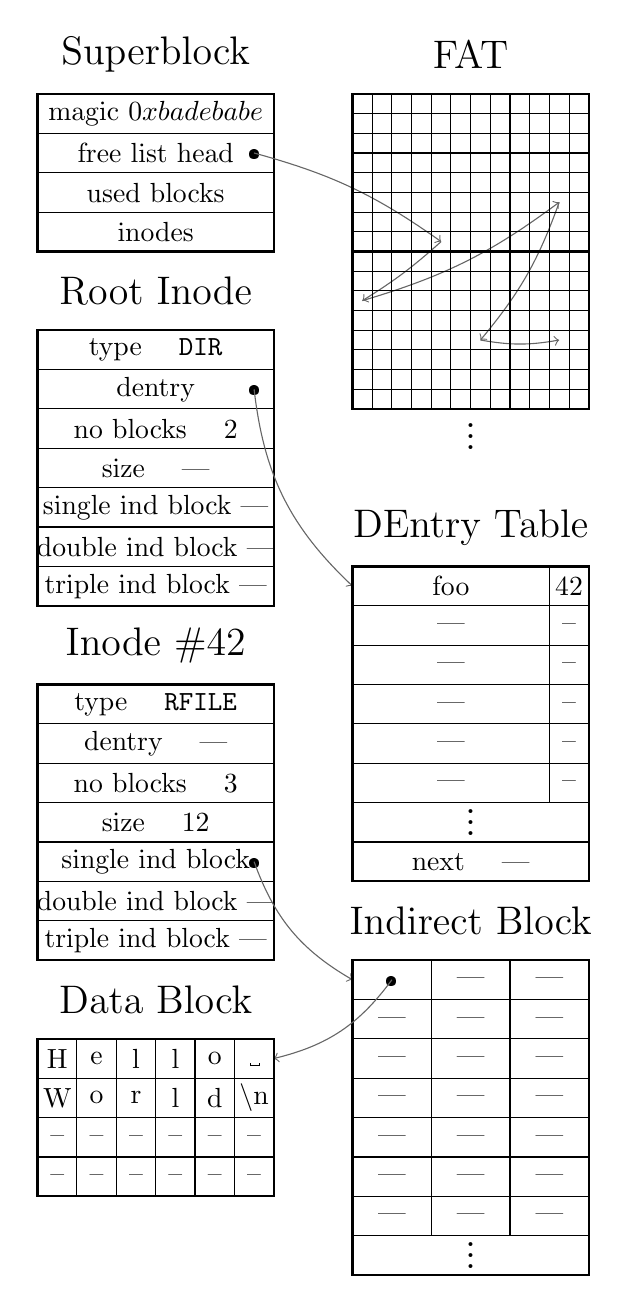
\begin{tikzpicture}[scale=1,outline/.style={draw=#1}]
      % \draw[help lines] (0,0) grid (8,16);
      
      \draw [thick] (0,13) rectangle (3,15);
      \draw (0,13.5) -- (3,13.5);
      \draw (0,14.0) -- (3,14.0);
      \draw (0,14.5) -- (3,14.5);

      \draw (1.5,14.75) node {magic $0\text{x}badebabe$};
      \draw (1.5,14.25) node {free list head};
      \draw (1.5,13.75) node {used blocks};
      \draw (1.5,13.25) node {inodes};

      \draw (2.75,14.42) node[anchor=north] {\textbullet};

      \draw[->, bend left=10, white!40!black] (2.75,14.25) to (5.125,13.125);

      \draw[->, bend left=5, white!40!black] (5.125,13.125) to (4.125,12.375);
      \draw[->, bend right=10, white!40!black] (4.125,12.375) to (6.625,13.625);
      \draw[->, bend left=10, white!40!black] (6.625,13.625) to (5.625,11.875);
      \draw[->, bend right=10, white!40!black] (5.625,11.875) to (6.625,11.875);

      \draw (1.5,15.5) node {\Large Superblock};

      \draw (5.5,15.5) node {\Large FAT};
      \draw [thick] (4,13) rectangle (7,15);
      \draw (5.5,10.75) node {\LARGE $\vdots$};
      \draw [thick] (4,11) rectangle (7,13);

      \foreach \y in {1,...,7} {
        \draw (4,13+0.25*\y) -- (7,13+0.25*\y);
      }

      \foreach \x in {1,...,11} {
        \draw (4+.25*\x,13) -- (4+.25*\x,15);
      }

      \foreach \y in {1,...,7} {
        \draw (4,11+0.25*\y) -- (7,11+0.25*\y);
      }

      \foreach \x in {1,...,11} {
        \draw (4+.25*\x,11) -- (4+.25*\x,13);
      }

      \draw (1.5,12.5) node {\Large Root Inode};
      \draw [thick] (0,8.5) rectangle (3,12);
      
      \draw (0,11.5) -- (3,11.5);
      \draw (0,11.0) -- (3,11.0);
      \draw (0,10.5) -- (3,10.5);
      \draw (0,10.0) -- (3,10.0);
      \draw (0,09.5) -- (3,09.5);
      \draw (0,09.0) -- (3,09.0);

      \draw (1.5,11.75) node {type \quad \verb|DIR|};
      \draw (1.5,11.25) node {dentry};
      \draw (1.5,10.75) node {no blocks \quad 2};
      \draw (1.5,10.25) node {size \quad ---};
      \draw (1.5,09.75) node {single ind block ---};
      \draw (1.5,09.25) node {double ind block ---};
      \draw (1.5,08.75) node {triple ind block ---};
      \draw (2.75,11.42) node[anchor=north] {\textbullet};

      \draw[->, bend right=20, white!40!black] (2.75,11.25) to (4,8.75);

      \draw (5.5,9.5) node {\Large DEntry Table};
      \draw [thick] (4,5) rectangle (7,9);

      \draw (4,5.5) -- (7,5.5);
      \draw (4,6.0) -- (7,6.0);
      \draw (4,6.5) -- (7,6.5);
      \draw (4,7.0) -- (7,7.0);
      \draw (4,7.5) -- (7,7.5);
      \draw (4,8.0) -- (7,8.0);
      \draw (4,8.5) -- (7,8.5);

      \draw (6.5,6.0) -- (6.5,9);

      \draw (5.5,5.85) node {\LARGE $\vdots$};
      \draw (5.5,5.25) node {next \quad ---};

      \draw (5.25,6.25) node {---};
      \draw (6.75,6.25) node {--};
      \draw (5.25,6.75) node {---};
      \draw (6.75,6.75) node {--};
      \draw (5.25,7.25) node {---};
      \draw (6.75,7.25) node {--};
      \draw (5.25,7.75) node {---};
      \draw (6.75,7.75) node {--};
      \draw (5.25,8.25) node {---};
      \draw (6.75,8.25) node {--};
      \draw (5.25,8.75) node {foo};
      \draw (6.75,8.75) node {42};

      \draw (1.5,8) node {\Large Inode \#42};
      \draw [thick] (0,4) rectangle (3,7.5);
      
      \draw (0,7.0) -- (3,7.0);
      \draw (0,11.0-4.5) -- (3,11.0-4.5);
      \draw (0,10.5-4.5) -- (3,10.5-4.5);
      \draw (0,10.0-4.5) -- (3,10.0-4.5);
      \draw (0,09.5-4.5) -- (3,09.5-4.5);
      \draw (0,09.0-4.5) -- (3,09.0-4.5);

      \draw (1.5,11.75-4.5) node {type \quad \verb|RFILE|};
      \draw (1.5,11.25-4.5) node {dentry \quad ---};
      \draw (1.5,10.75-4.5) node {no blocks \quad 3};
      \draw (1.5,10.25-4.5) node {size \quad 12};
      \draw (1.5,09.75-4.5) node {single ind block};
      \draw (1.5,09.25-4.5) node {double ind block ---};
      \draw (1.5,08.75-4.5) node {triple ind block ---};

      \draw (2.75,09.75-4.5+.17) node[anchor=north] {\textbullet};

      \draw[->, bend right=20, white!40!black] (2.75,09.75-4.5) to (4,3.75);


      \draw (5.5,9.5-5) node {\Large Indirect Block};
      \draw [thick] (4,5-5) rectangle (7,9-5);

      \draw (4,5.5-5) -- (7,5.5-5);
      \draw (4,6.0-5) -- (7,6.0-5);
      \draw (4,6.5-5) -- (7,6.5-5);
      \draw (4,7.0-5) -- (7,7.0-5);
      \draw (4,7.5-5) -- (7,7.5-5);
      \draw (4,8.0-5) -- (7,8.0-5);
      \draw (4,8.5-5) -- (7,8.5-5);

      \draw (5,4) -- (5,0.5);
      \draw (6,4) -- (6,0.5);

      \draw (5.5,09.25-4.5-1.0) node {---};
      \draw (5.5,09.25-4.5-1.5) node {---};
      \draw (5.5,09.25-4.5-2.0) node {---};
      \draw (5.5,09.25-4.5-2.5) node {---};
      \draw (5.5,09.25-4.5-3.0) node {---};
      \draw (5.5,09.25-4.5-3.5) node {---};
      \draw (5.5,09.25-4.5-4.0) node {---};

      \draw (6.5,09.25-4.5-1.0) node {---};
      \draw (6.5,09.25-4.5-1.5) node {---};
      \draw (6.5,09.25-4.5-2.0) node {---};
      \draw (6.5,09.25-4.5-2.5) node {---};
      \draw (6.5,09.25-4.5-3.0) node {---};
      \draw (6.5,09.25-4.5-3.5) node {---};
      \draw (6.5,09.25-4.5-4.0) node {---};

      \draw (4.5,09.25-4.5-1.5) node {---};
      \draw (4.5,09.25-4.5-2.0) node {---};
      \draw (4.5,09.25-4.5-2.5) node {---};
      \draw (4.5,09.25-4.5-3.0) node {---};
      \draw (4.5,09.25-4.5-3.5) node {---};
      \draw (4.5,09.25-4.5-4.0) node {---};

      \draw (5.5,5.85-5.5) node {\LARGE $\vdots$};

      \draw (4.5,09.25-4.5-1.0+.17) node[anchor=north] {\textbullet};

      \draw[->, bend left=20, white!40!black] (4.5,09.25-4.5-1.0) to (3,2.75);

      \draw (5.5-4,15.5-12) node {\Large Data Block};
      \draw [thick] (0,1) rectangle (3,3);

      \foreach \y in {1,...,3} {
        \draw (0,1+0.5*\y) -- (3,1+0.5*\y);
      }

      \foreach \x in {1,...,5} {
        \draw (.5*\x,1) -- (.5*\x,3);
      }

      \draw (0.25,2.75) node {H};
      \draw (0.75,2.75) node {e};
      \draw (1.25,2.75) node {l};
      \draw (1.75,2.75) node {l};
      \draw (2.25,2.75) node {o};
      \draw (2.75,2.675) node {\textvisiblespace};

      \draw (0.25,2.25) node {W};
      \draw (0.75,2.25) node {o};
      \draw (1.25,2.25) node {r};
      \draw (1.75,2.25) node {l};
      \draw (2.25,2.25) node {d};
      \draw (2.75,2.25) node {\textbackslash n};

      \draw (0.25,1.75) node {--};
      \draw (0.75,1.75) node {--};
      \draw (1.25,1.75) node {--};
      \draw (1.75,1.75) node {--};
      \draw (2.25,1.75) node {--};
      \draw (2.75,1.75) node {--};

      \draw (0.25,1.25) node {--};
      \draw (0.75,1.25) node {--};
      \draw (1.25,1.25) node {--};
      \draw (1.75,1.25) node {--};
      \draw (2.25,1.25) node {--};
      \draw (2.75,1.25) node {--};

    \end{tikzpicture}
    \caption{\pfs Example of \pfsfs Structure.}
    \label{fig:pfsstructex}
  \end{center}
\end{figure}

\section{Implementation}
The implementation of \pfsfs tries to be as minimalist as possible.
There were no special concerns with seek times and the number of
disk accesses, except in critical operations such as \verb|read()|
and \verb|write()|. There are lots of room left for optimizations,
such as caching.

The \pfs file system has a block size of $1024$ bytes. This value
was used to balance a tradeoff between internal fragmentation,
number of access to read/write data and the size of the file allocation 
table (which end up being $\sim16$MB). This block size can easily be
changed but this was the only size which was tested. 

To simplify the manipulation of dentry table a directory always
have at least one dentry table. When a file is created in a directory
the first empty slot in the list of dentry table is used to store
that file. When a file is removed the correspondent dentry table
may get empty. In such cases that dentry table is freed (unless it is the
first one) and the previous table will point to the next. 
A slot is empty when the filename has length zero.
The filename is stored in a nul terminated string, making the maximum
file name $63$ bytes long. Each dentry table has $15$ entries.

Every regular file always have a single indirect block. Each indirection 
has $256$ pointers. This means that with only one indirection a file
have a maximum of $256 \cdot 1024 \, \text{bytes} = 256\text{KB}$.
The usage of double indirect block allows this limit to be 
$256 \cdot 1024 + 256^2 \cdot 1024 \, \text{bytes} = \sim64\text{MB}$
and a triple indirect block expand the limit far beyond the
maximum file system size: 
$256 \cdot 1024 + 256^2 \cdot 1024  + 256^3 \cdot 1024 \, \text{bytes} 
= \sim16\text{GB}$.

To create a valid \pfsfs in a device a formatting tool was developed.
This tool writes the initial state expected in a empty file system.
Since no attention was made to normalize the endianness of integer
values the portability of the \pfsfs only hold for system using
the same endianness. (An attempt to do otherwise will result in the
magic number mismatch and the file system will refuse to mount, causing
to harm to the file system.)

The operations implemented were \verb|mkdir()|, \verb|opendir()|, \\
\verb|readdir()|, \verb|closedir()|, \verb|rmdir()/unlink()|,
\verb|rename()|, \\ \verb|open()/creat()|, \verb|read()|, \verb|write()|,
\verb|close()|, \verb|truncate()|, \verb|access()|, \verb|getattr()| and
\verb|statfs()|.

Since not all operation can be done in open file a red-black tree maintains
a counter for each opened file. The only operation that cannot be done
on an open regular file is \\ \verb|unlink()|, which will return \verb|EBUSY|
if done on a file which is opened. Other operations such as \verb|rename()|
can be done on open files since the inode remains unchanged. There is
no problem in removing directories since the file system will be able to
detect that and return a proper error to a process reading the directory 
(because the \verb|readdir()| is atomic).

All operations are atomic using reentrant mutexes to enforce mutual exclusion.

\section{Evaluation}
To evaluate \pfsfs a series of stress test were performed.

To test the overall file system usage under lots of files of relatively
small size the \verb|linux-3.0.8.tar.bz2| was copied into the file system
and extracted. The tarball itself have $74$ MB, thus forcing the
triple indirect block to be used. The \emph{md5sum} of the tarball 
matched the expected result. The tarball was then extracted
creating $39055$ files. The directory structure was preserved and 
the \emph{md5sum} of every file was ok\footnote{There was only one missing file
which was a soft-link, which are not supported in \pfsfs}.
The exact same procedure was done with \verb|gcc-4.6.2.tar.bz2| with
successful result except for $60$ java compiled files with filenames
larger than supported.

To test large files a few TV series were copied to the disk. 
The \emph{md5sum} was also correct. The whole file system were filled
with 4GB of TV series, my personal git repository ($\sim630$MB) and
some photos. As expected the trying to copy more files gave a 
``no space left on device'' error. After the removal of all these files
the file system reported a usage of $\sim1\%$, the minimum taking into account
the file allocation table size. To test even larger files the
Star Wars Episode I --- The Phantom Menace\footnote{I apologize for not 
  using the Episode IV.}, with $\sim1.5$GB was copied to
the file system and the \emph{md5sum} gave the correct result. 
MPlayer was also able to play it correctly and with no noticeable delay.

The \verb|truncate()| operations was also tested by expanding
and shrinking files, with the result compared to the same operations done
on a \emph{ext4} file system giving the same result.

% evaluation
%   multi directory, many small files:
%     copied linux-3.0.8.tar.bz2 . md5sum ok
%     extract linux-3.0.8.tar.bz2 with 39055 files
%     computed md5sums
%     downloaded gcc-4.6.2.tar.bz2 with to FS. md5sum ok
%     extracted gcc-4.6.2.tar.bz2 with 75903 files
%     md5 ok, except for 60 java compliled files with filenames >= 64
%   large files
%     Star Wars Quote: a long long file in a block far far away
%       Star\ Wars/Episode\ 1-The\ Phantom\ Menace (pedir desculpa de nao começar 
%       por pelo ep IV)
%       1.5GB. md5 ok. mplayer ok
%   - random access
%   disk full
%     ok
%   IOZone

\section{Conclusion}
Building a file system from scratch was very interesting and allowed me
to better understand some of the fundamental data structures used in
file system design. Since the \pfs was designed to have acceptable
``real world'' restrictions it was also very rewarding to see some
normal common tasks being done in the file system.

\bibliographystyle{abbrv}
\bibliography{report}

\end{document}
